\section{Architectural design}

\subsection{Overview}
	\subsubsection{Context viewpoint}
	
		\begin{figure}[h!]
			\centering
			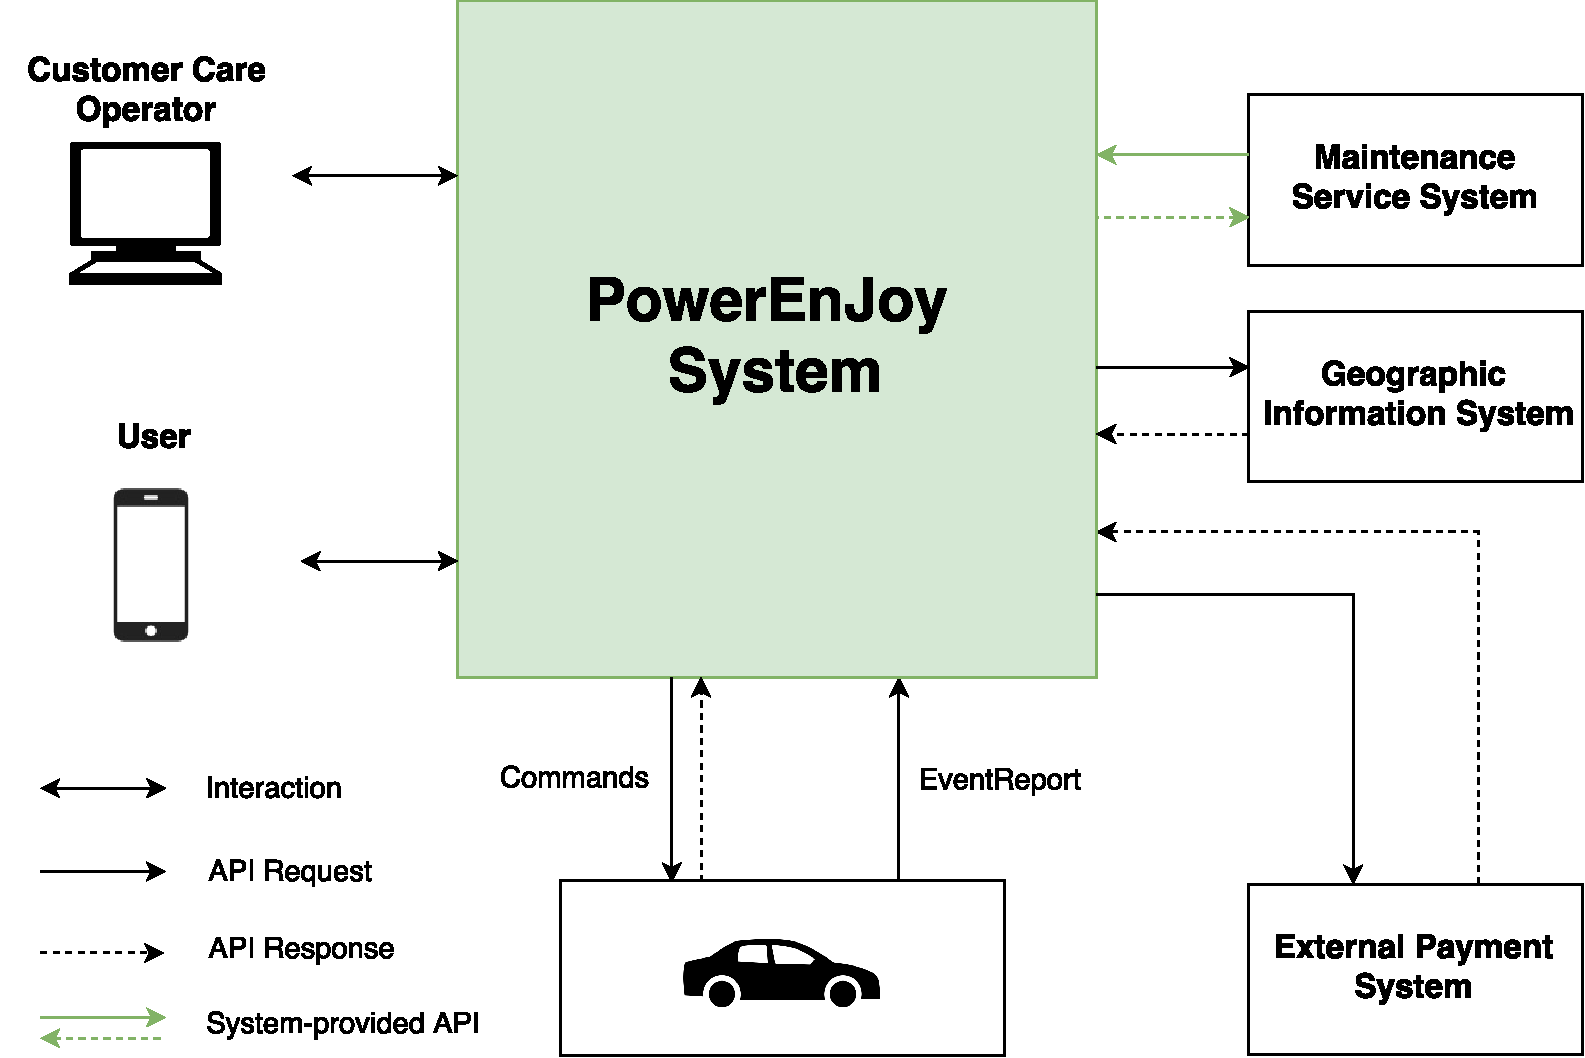
\includegraphics[width=\linewidth]{contextViewPoint}
			\caption{
				\label{fig:contextViewPoint} 
				Context viewpoint
			}
		\end{figure}
		
		We need to design a system which allows communications with many agents such as cars, users, external systems, etc.
		Moreover we recognize that in most of the interactions the system is providing a service to agents so, after taking in consideration different alternatives, we decided to use a client-server architectural approach.
		
		Cars offer to the system a set of primitives which allow it to interact with them: in this case it is clear that cars are providing the system services, so they can be identified as serves while the system acts as a client; on the other end the notification functionality offered by cars clearly yields to an event-based approach due to the asynchronous nature of such interactions, this led us to use a publish-subscribe paradigm for these specific interactions.
		\clearpage
		
	\subsubsection{Composition viewpoint}
	
		\begin{figure}[h!]
			\centering
			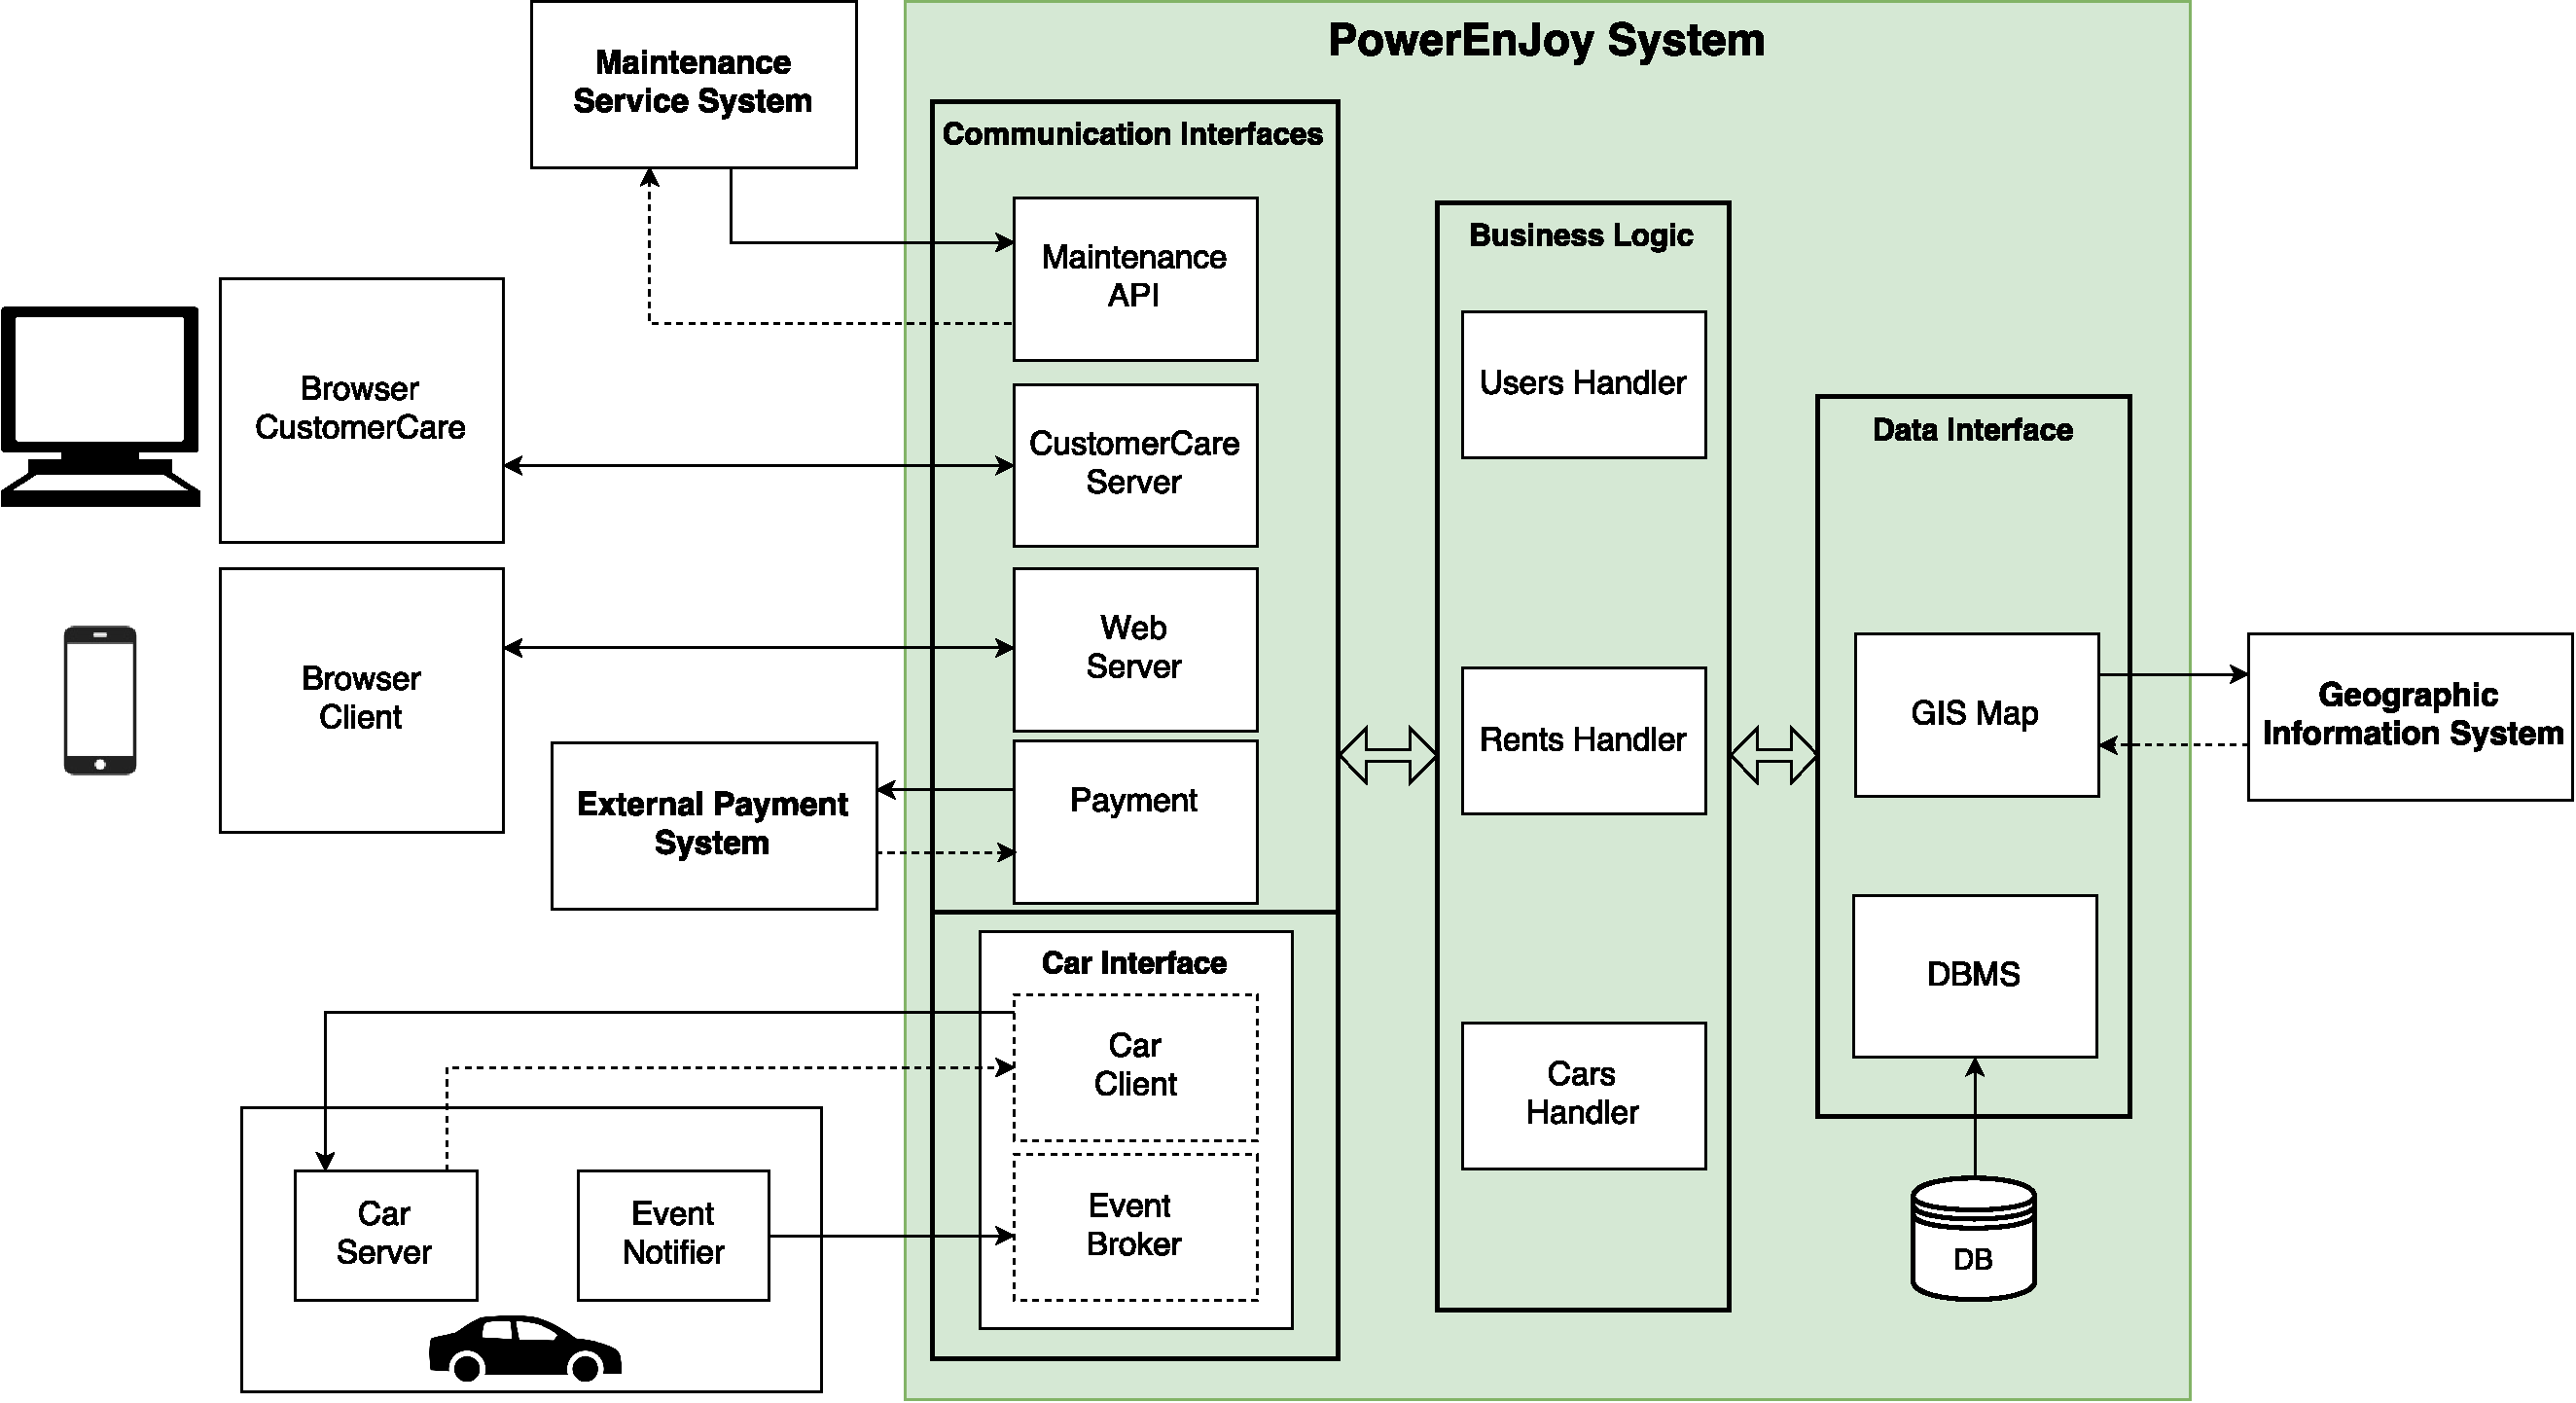
\includegraphics[width=\linewidth]{ComponentOverview}
			\caption{
				\label{fig:contextViewPoint} 
				Context viewpoint
			}
		\end{figure}
		
		

\subsection{Component view}
\subsection{Deployment view}
\subsection{Runtime view}
\subsection{Component interfaces}
\subsection{Architectural style and patterns}
\subsection{Other design decision}
